\documentclass[12pt,a5paper]{article}
\usepackage{amsmath,natbib,defns,reducecode}
\IfFileExists{ajr.sty}{\usepackage{ajr}}{}
\title{Ensure continuity and self-adjointness of holistic discretisation of (n)lS equation with periodic potential wells}
\author{AJR}
\date{\today}

\begin{document}

\maketitle

Execute in Reduce with \verb|in_tex "potwell.tex"$|

Instead of the nlS, start by modelling the 1D diffusion \pde\ with potential wells \(V(x):=-\frac{A\pi^2}{H^2}\cos(2\pi x/H)\),
\begin{equation*}
-i\D tu=\DD xu-V(x)u
\end{equation*}
on a macroscale grid with same spacing as the wells: that is, locate the grid at the minimum of the wells at \(X_j=jH\) say.
The \(j\)th~element is \(X_{j-1}\leq x\leq X_j\).

\begin{figure}
\centering
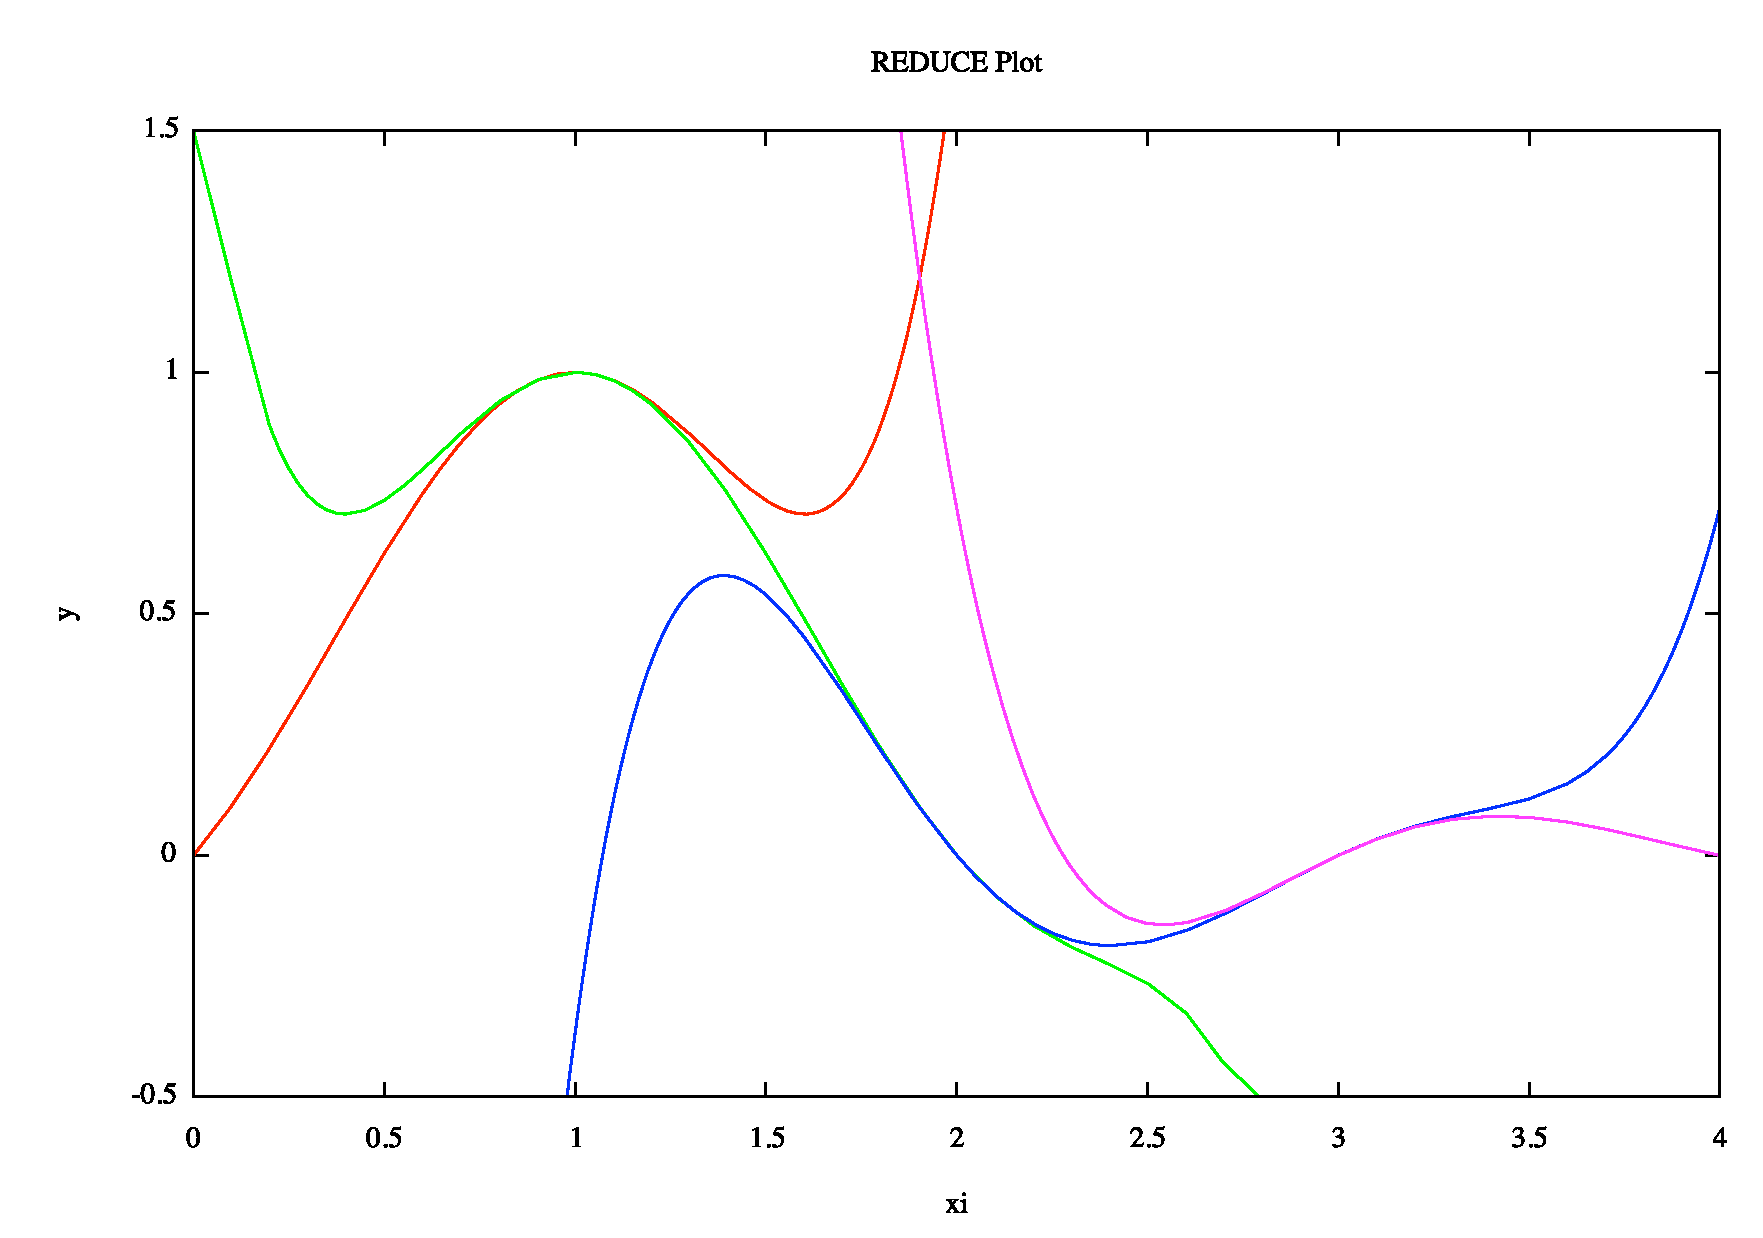
\includegraphics[width=\linewidth]{A0gam3}
\caption{beautiful \(C^2\), piecewise quintic, approximation to the subgrid fields of the `diffusion' \pde, \(A=0\)\,, with coupling errors~\Ord{\gamma^3}: red, \(0\leq\xi\leq1\); green, \(1\leq\xi\leq2\); blue, \(2\leq\xi\leq3\); magenta, \(3\leq\xi\leq4\).}
\label{fig:A0gam3}
\end{figure}

\begin{figure}
\centering
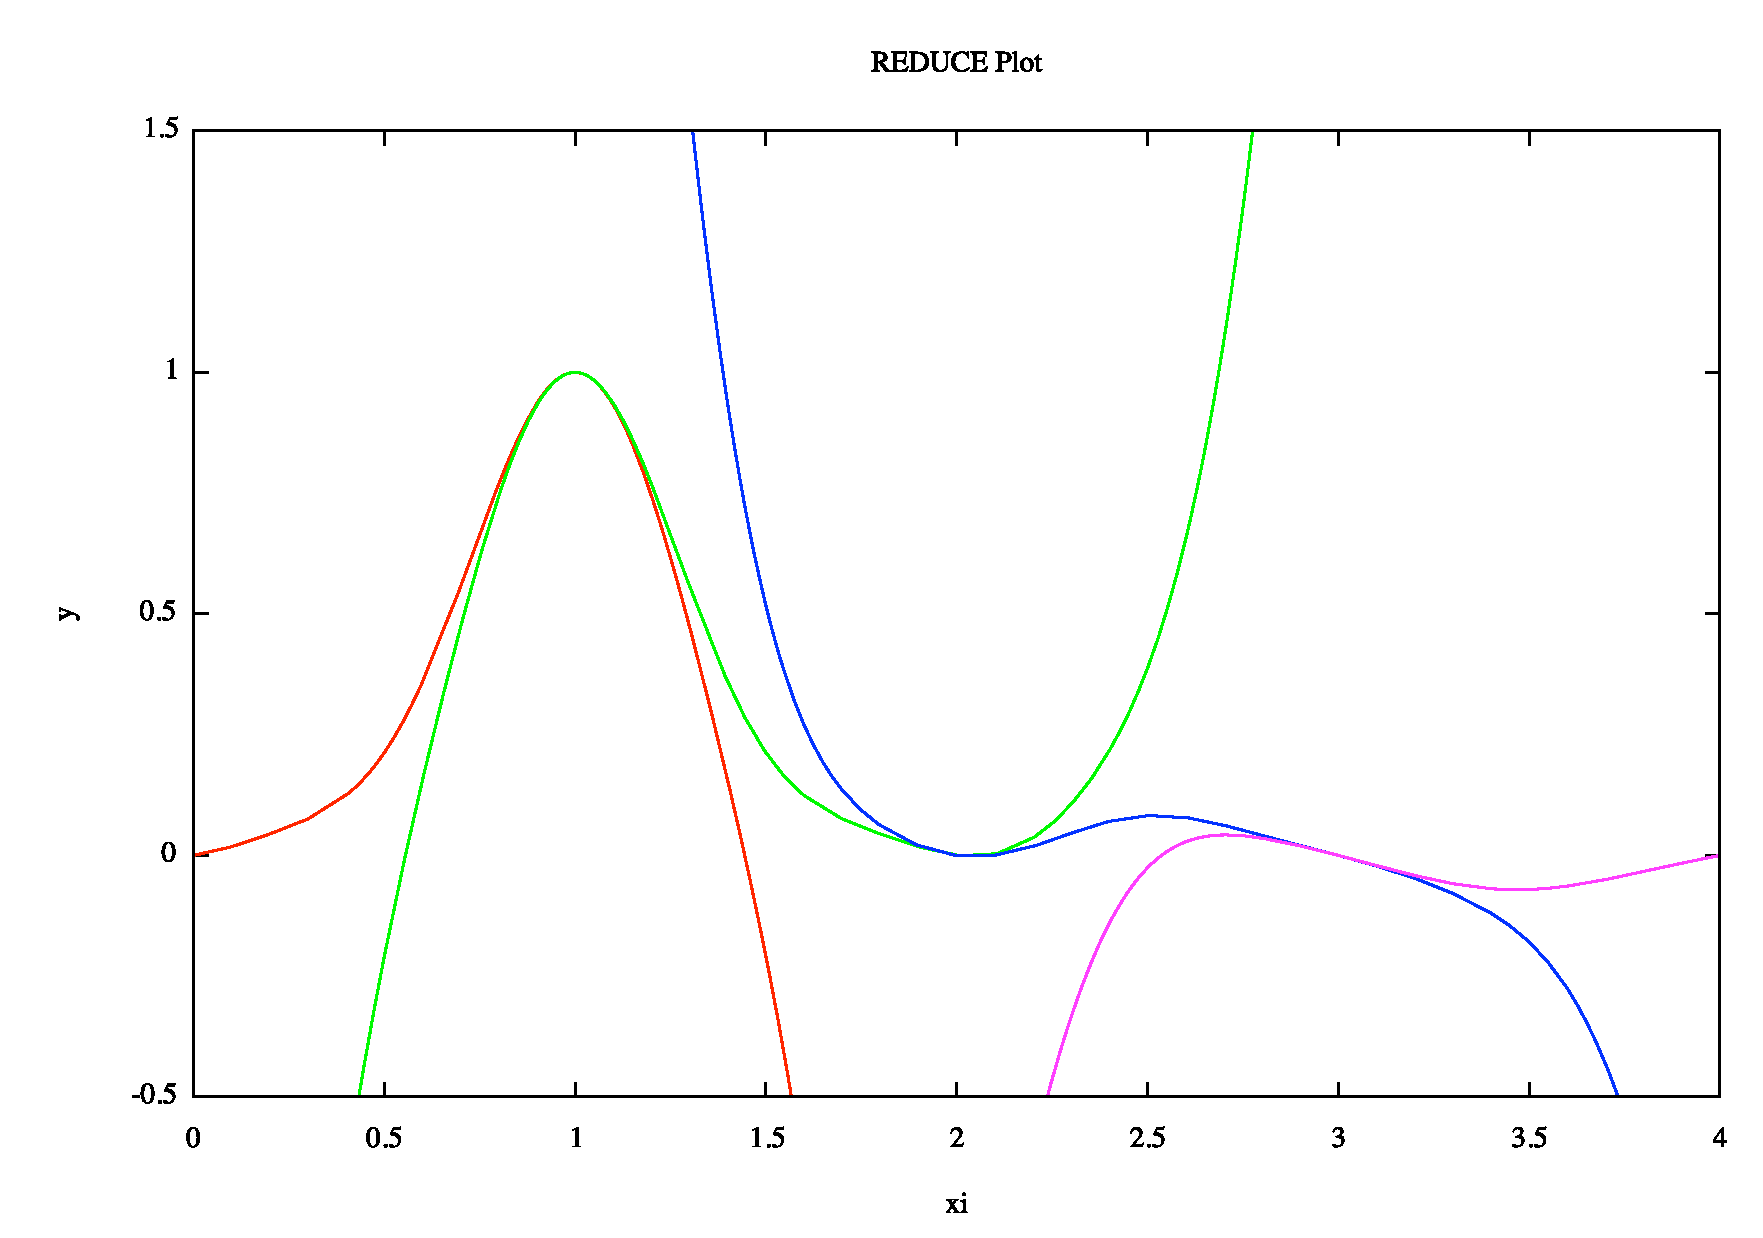
\includegraphics[width=\linewidth]{A1gam2}
\caption{beautiful \(C^2\) approximation to the subgrid fields of the  \pde\ with potential strength \(A=1\) and coupling errors~\Ord{\gamma^2} (should only be~\(C^1\)!): red, \(0\leq\xi\leq1\); green, \(1\leq\xi\leq2\); blue, \(2\leq\xi\leq3\); magenta, \(3\leq\xi\leq4\).  }
\label{fig:A1gam2}
\end{figure}


Improve printing.
\begin{reduce}
on div; off allfac; on revpri;
factor hh,uu,d,aa;
\end{reduce}

Define shift right/left operators \verb|ep| and~\verb|em|: use that in terms of centred mean and difference operators, \(\mu\)~and~\(\delta\), they are \(1\pm\mu\delta+\rat12\delta^2\) \cite[p.65]{npl61}.
Also encode the identity that \(\mu^2=1+\delta^2/4\)\,.
Define the `spline' operator \(\verb|ss|=S:=(1+\delta^2/6)^{-1}\).
Have verified that, on an infinite lattice, operator~\(S\) is the Toeplitz matrix with elements
\begin{equation*}
S_{ij}=\sqrt3(-2+\sqrt3)^{|i-j|}=\sqrt3(- 0.2679)^{|i-j|}.
\end{equation*}
\begin{reduce}
ep:=1+mu*del+del^2/2;
em:=1-mu*del+del^2/2;
let { mu^2=>1+del^2/4
    , ss*del^2=>6-6*ss };
\end{reduce}

Write the solution in terms of the microscale variable~\(\xi:=(x-X_{j-1})/H\).
\begin{reduce}
depend xi,x; 
let df(~a,x)=>df(a,xi)/hh;
\end{reduce}

To find corrections, linear operator~\verb|linv| solves \textsc{de}s of the form \(\DD \xi{\hat u}=\text{Res}\) such that \(\hat u=0\) at \(\xi=0,1\).
\begin{reduce}
operator linv; linear linv;
let { linv(xi^~~p,xi)=>(xi^(p+2)-xi)/(p+1)/(p+2)
    , linv(1,xi)=>(xi^2-xi)/2 
    , linv(cos(~~m*pi*xi),xi)
        =>(1-cos(m*pi*xi))/(m*pi)^2 when evenp(m)
    , linv(sin(~~m*pi*xi),xi)=>-sin(m*pi*xi)/(m*pi)^2 
    , linv(xi^~~p*cos(~~m*pi*xi),xi)
        =>xi^p*(1-cos(m*pi*xi))/(m*pi)^2 when evenp(m)
    , linv(xi^~~p*sin(~~m*pi*xi),xi)
        =>-xi^p*sin(m*pi*xi)/(m*pi)^2 
    };
\end{reduce}

Write the slow manifold in terms of amplitudes \(U_j(t):=u(X_j,t)\).  
These depend upon time according to \(\de t{U_j}=g_j\)\,.
We let all the \(j\)~dependence be in the operators.
\begin{reduce}
depend uu,t; 
let df(uu,t)=>g;
\end{reduce}

The linear solution are equilibria, \(g=0\), of piecewise linear field between \(U_{j-1}\) at \(\xi=0\) and \(U_j\) at \(\xi=1\).
\begin{reduce}
g:=0;
u:=xi*uu+(1-xi)*em*uu;
\end{reduce}

Iterate until the slow manifold model is found to the following specified order of accuracy.
\begin{reduce}
let { gamma^2=>0, aa^2=>0 };
for it:=1:99 do begin 
\end{reduce}

Compute residuals of governing equations.
\begin{reduce}
    pde:=trigsimp(
        i*df(u,t)+df(u,x,x)+aa*pi^2/hh^2*cos(2*pi*xi)*u
        , combine);
    amp:=sub(xi=1,u)-uu;
    cty:=sub(xi=0,ep*u)-sub(xi=1,u);
    hux:=hh*df(u,x)$
    jmp:=-sub(xi=0,ep*hux)+sub(xi=1,hux)
        +(1-gamma)*sub(xi=1,ep*u-2*u+em*u);
    write lengthRes:=map(length(~a),{pde,amp,cty,jmp});
\end{reduce}

Correct approximations based upon the residuals.
These ad hoc corrections are not optimal, but they do work after enough iterations.
\begin{reduce}
    g:=g+i*(gd:=-ss*jmp/hh^2);
    u:=u-linv(pde-(xi+(1-xi)*em)*gd,xi)*hh^2;
\end{reduce}

Exit the loop when all residuals are zero to the order specified.
\begin{reduce}
    showtime;
    if {pde,amp,cty,jmp}={0,0,0,0} then write it:=it+10000;
end;
\end{reduce}


Confirm left-right symmetry.
\begin{reduce}
v:=trigsimp(sub({del=-del,xi=1-xi},ep*u))$
duv:=trigsimp(v-u);
\end{reduce}

Get equivalent \pde, but need to improve to be able to analyse to any order.
Here, \verb|d| denotes~\(\D x{}\).
\begin{reduce}
mig:=-i*g;
ssd:=1-hh^2*d^2/6+hh^4*d^4/72-hh^6*d^6/2160;
let d^7=>0;
migde:=sub(ss=ssd,-i*g);
\end{reduce}

%This appears to simplify the form of the evolution:
%introducing \(\verb|gamdel2|:=\gamma\delta^2\).
%\begin{reduce}
%factor gamdel2;
%g:=(g where ss*gamma=>gamma-ss/6*gamdel2);
%u:=(u where { ss*gamma=>gamma-ss/6*gamdel2
%            , gamma*del^2=>gamdel2})$
%\end{reduce}
Optionally plot some fully coupled subgrid fields of the linear problem, \(\epsilon=0\)\,, for a potential strength \(A=1\), say.
Result is beautiful.
\begin{reduce}
load_package gnuplot;
if 1 then begin
hh:=1; gamma:=1; epsilon:=0; aa:=1;
u:=(sub(mu=delmu/del,u) where del^2=>delsq);
off nat;out "tmp.red"$
write u:=u$
write g:=g$
write "end;"$
shut "tmp.red"$ on nat;
n:=20; % 20 may be enough, but increase to test
matrix ss(2*n-1,2*n-1),delsq(2*n-1,2*n-1),delmu(2*n-1,2*n-1),uu(2*n-1,2*n-1);
for i:=1:2*n-1 do 
    for j:=1:2*n-1 do 
        ss(i,j):=sqrt(3)*(-2+sqrt(3))^abs(i-j);
for i:=1:2*n-1 do uu(i,i):=1;
for i:=1:2*n-1 do delsq(i,i):=-2;
for i:=2:2*n-1 do delsq(i,i-1):=delsq(i-1,i):=1;
for i:=2:2*n-1 do delmu(i,i-1):=-1/2;
for i:=2:2*n-1 do delmu(i-1,i):=+1/2;
on rounded; print_precision 4;
in "tmp.red";
ujs:=map(max(-1/2,min(3/2,~a)),
      {u(n,n)
      ,sub(xi=xi-1,u(n+1,n))
      ,sub(xi=xi-2,u(n+2,n))
      ,sub(xi=xi-3,u(n+3,n))
      });
plot(ujs,xi=(0 .. 4));
end;
\end{reduce}

Fin.
\begin{reduce}
end;
\end{reduce}

\bibliographystyle{agsm}
\bibliography{bibexport,bib}

\end{document}
